\documentclass[]{article}
\usepackage[]{graphicx} 
\usepackage[utf8]{inputenc} 
\usepackage[OT1]{fontenc} 
\usepackage[]{subcaption} 
\usepackage{simplewick}
\usepackage{caption}
\usepackage{amsmath}
\usepackage[]{mathtools} 
\usepackage[]{amssymb} 
\usepackage{prettyref}
\newrefformat{fig}{Figure~[\ref{#1}]}

\begin{document}

\title{Introduction To Reinforcement Learning}
\author{Felipe Glicério Gomes Marcelino}
\date{18 April 2020}
\maketitle

\subsection*{Slide 3}%
\label{sub:Slide 3}

\subsubsection*{Today's Lecture}

\begin{enumerate}
    \item Definition of a Markov decision process
    \item Description of reinforcement learning problem
    \item Anatomy of an RL algorithm
    \item A brief overview of RL algorithm types
\end{enumerate}

\begin{itemize}
    \item Goals:
        \begin{itemize}
            \item Understand definitions \& notation
            \item Understand the underlying reinforcement learning objective
            \item Get a summary of possible algorithms
        \end{itemize}
\end{itemize}

\subsection*{Slide 4}%
\label{sub:Slide 4}

Some observations:
\begin{itemize}
    \item Behavioral Cloning works with partial observations ($o_{t}$), but
    \item Dagger assumption about the error  $\epsilon $ is only possible with thoroughly observations states ($s_{t}$)
\end{itemize}

\subsection*{Slide 5}%
\label{sub:Slide 5}

\subsubsection*{Reward functions}

\begin{itemize}
    \item Reward functions tell us which states and actions are better.
    \item Finds out a good reward function is one of the most challenging problems in reinforcement learning.
    \item Objective: Taking actions that will maximize long-term rewards rather than rewards at immediate next
        step
    \item Markov decision process definition: $s, a, r(s,a), p(s'|s,a)$
\end{itemize}

\subsection*{Slide 8}
\label{sub:Slide 8}

\subsubsection*{Markov Chain}
\label{sub:Markov Chain}

Definitions: 
\par 


\begin{tabular}{ccc}
    $\mathit{M}= \{S, T\}$ & & \\
    $\mathit{S} - \text{State Space}$ & states $s \in S$ (discrete or continuous) & \\
    $\tau - \text{Transition Operation}$ & $p(s_{t + 1}|s_{t})$ &  (1)\\
    $\mu_{t,i} = p(s_{t} = i)$ & Probability of being in state I at time step T &  (2)\\
    $\mathit{T_{i,j}} = p(s_{t + 1} = i | s_{t} = j)$ & (3) &  (4)\\
\end{tabular}


\begin{itemize}
    \item (1) - Probability of go to the state $s_{t+1} $ from $s_{t}$
    \item (2) - $\vec{\mu_{t}}$ is a vector of probabilities
    \item (3) - Matrix - Probability of going at a state $i$ given that currently state J
    \item (4) - then $\vec{\mu_{t+1}} = \tau\vec{\mu_{t}}$
\end{itemize}

\begin{figure}
\begin{center}
    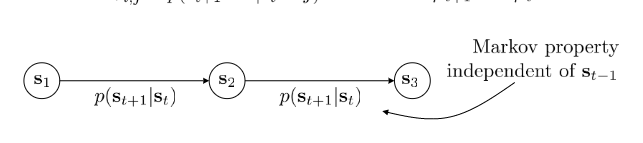
\includegraphics[scale=0.5]{cap3img/markovchain.png}.png
\end{center}
\caption{Markov Chain}
\label{fig:markovchain}
\end{figure}

\prettyref{fig:markovchain} shows how is a markov chain graphic model. 



\subsection*{Slide 9 - 10}
\label{sub:Slide 9}

\subsubsection*{Markov Decision Process}
\label{sub:Markov Decision Process}


Defitions:
\par 
\begin{tabular}{ccc}
    $\mathit{S}$ - state space & states $s \in S$ (discrete or continuous ) & \\
    $\mathit{A}$ - action space & actions $a \in A$ (discrete or continuous) & \\
    $\tau$ - transition operator (Tensor: 3D) & & \\
    let $\mu_{t,j} = p(s_{t} = j)$ & $\mu_{t,i}= \sum_{j,k}\tau_{i,j,k}\mu_{t,j}\xi_{t,k}$ & \\
    let $\xi_{i,k} = p(a_{t} = k)$ & & \\
    let $\tau_{i,j,k} = p(s_{t + 1} = i | s_{t} = j, a_{j} = k)$
    $\mathit{r}$ - reward function  & $r : \mathit{S} \times \mathit{A} \rightarrow \mathbb{R}$ & \\
                                    & $r(s_{t},a_{t})$ - reward & \\
\end{tabular}

\begin{figure}
\begin{center}
    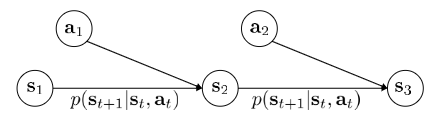
\includegraphics[scale=0.5]{cap3img/markovprocess.png}
\end{center}
\caption{Markov Process}
\label{fig:markovprocess}
\end{figure}



\subsection{Slide 12-14}%
\label{sub:Slide 12}

\begin{figure}
\begin{center}
    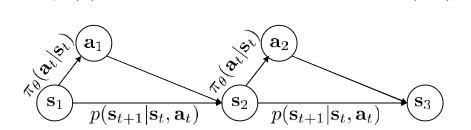
\includegraphics[scale=0.5]{cap3img/markovchaincomp.png}
\end{center}
\caption{Markov chain with augmentation state space}
\label{fig:markovprocesscomp}
\end{figure}

\prettyref{fig:markovprocess} and \prettyref{fig:markovprocesscomp} show how is a markov process graphic model and
markov chain with augmentation state space.

The goal of reinforcement learning. Markov decision giving us:

$$\underbrace{p_{\theta}(s_{1},a_{1},\cdots, s_{T},a_{T})}_{p_\theta(\tau)} = \underbrace{p(s_{1}) \prod_{t=1}^{T}\pi_{\theta}(a_{t}|s_{t})p(s_{t +
    1}|s_{t},a_{t})}_{\text{Markov chain on}  (s,a)}$$

$\tau$ is a trajectory. It is easy to see that adding the policy inside $\prod$, the MDP models transforms into a Markov
chain. Using the above, we want to find out the best parameters to maximize the expectation of reward:

$$\theta^{*} = \underset{\theta}{argmax}\mathit{E}_{\tau \sim p_{\theta}(\tau)} = \left[ \sum_{t} r(s_{t},a_{t})
\right]$$

\par Using the MDP definition above, all actions are possible in all states. But, it is possible to put negative rewards
when some actions are illegal given a specific state. Or maybe remap illegal actions to do something else.

\textbf{Tip}: 
$$ E_{x\sim p(x)}[f(x)] = \int p(x)f(x)dx $$

\par Redefining the state space to group the S and A, it is possible using the graphic model in
\prettyref{fig:markovprocesscomp3}(Markov Chain). So the probability of next the state and the next action given the current
state and current action is just obtained by multiplying together  transition dynamics of the original MDP and the
policy.


\begin{figure}
\begin{center}
    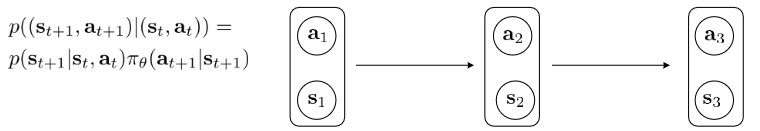
\includegraphics[scale=0.5]{cap3img/markovprocess3.png}
\end{center}
\caption{Markov chain notation using A and S space together.}
\label{fig:markovprocesscomp3}
\end{figure}

\subsection*{Slide 15}%
\label{sub:Slide 15}

\subsubsection*{Finite Horizon Case: State-Action Marginal}
\label{sub:Finite Horizon Case: State-Action Marginal}

\begin{gather}
    \begin{align}
    \theta^{*} = \underset{\theta}{argmax}\mathit{E}_{\tau \sim p_{\theta}(\tau)} = \left[ \sum_{t} r(s_{t},a_{t})\right]  \\
    \theta^{*} =\underset{\theta}{\text{argmax}}\sum_{t=1}^{T}\mathit{E_{(s_{t},a_{t})\sim p_{\theta}(s_{t},a_{t})[}} [r(s_{t},a_{t})] 
    \end{align}
\end{gather}


\begin{figure}
\begin{center}
    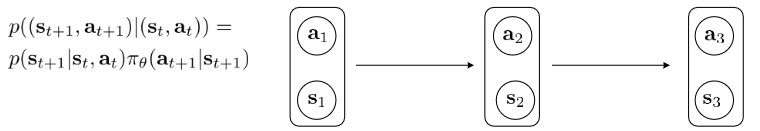
\includegraphics[scale=0.5]{cap3img/transition.png}
\end{center}
\caption{Transition Operation}
\label{fig:transition}
\end{figure}


\par $\mathit{E}$ can be pushed inside the $\sum$, by the linearity of expectations propriety. And because of the term inside the sum
only depends on $s_{t}$ and $a_{t}$, I can rewrite it. Rather than having it be an expectation over all trajectories, I
can have it be expectation over just  $s_{t}$ and $a_{t}$, which calls state action marginal $\rightarrow
p_{\theta}(s_{t},a_{t})$

\subsection*{Slide 16}%
\label{sub:Slide 16}

\subsubsection*{Infinite Horizon case: Stationary Distribution}
\label{sub:Infinite Horizon case: Stationary Distribution}
\par Now, if $\mathit{T}$ = $\infty$ ? Considering:

\begin{equation}
    \label{eq:stationary}
    \theta^{*} =\underset{\theta}{\text{argmax}}\sum_{t=1}^{T}\mathit{E_{(s_{t},a_{t})\sim p_{\theta}(s_{t},a_{t})[}} [r(s_{t},a_{t})] 
\end{equation}


\begin{align}
    \label{eq:mu}
    \mu & = \begin{bmatrix}
        $$p(s_{1},a_{1})$$ \\
        $$p(s_{1},a_{2})$$ \\
        \vdots \\
        $$p(s_{1},a_{m})$$ \\
        $$p(s_{2},a_{1})$$ \\
        \vdots \\
            \end{bmatrix}
\end{align}

\par $p(s_{t},a_{t})$ converges to a stationary distribution. Therefore, $\mu=\tau\mu$. Solving $(\tau - 
\mathbb{I})\mu = 0$ results in Stationary Distribution. \textbf{OBS:} $\mu$ is an eigenvector of $\tau$.  It means that the
distribution over $\mu$ doesn't change after a transition. $\mu = p_{\theta}(s,a) \leftarrow$ Stationary distribution.
\par 
As T goes to $\infty$ in \eqref{eq:stationary}, the sum is dominated by terms of the stationary distribution. However, the
result of the $\sum$ over $\infty$ is $\infty$. So, it is necessary to adding a new term to have a well-defined answer and sum up
to something finite. The term
is $\frac{1}{T}$. It is called \textbf{Undiscounted Average Return Formulation of RL}. Then the optimal policy can be
represented as follows:

\begin{equation}
    \label{eq:stationary2}
    \theta^{*} =\underset{\theta}{\text{argmax}}\frac{1}{T}\sum_{t=1}^{T}\mathit{E_{(s_{t},a_{t})\sim p_{\theta}(s_{t},a_{t})[}}
    [r(s_{t},a_{t})]  \rightarrow \mathit{E}_{(s,a) \sim p_{\theta}(s,a)}[r(s,a)]
\end{equation}

\subsection*{Slide 18}%
\label{sub:Slide 18}

\begin{figure}
\begin{center}
    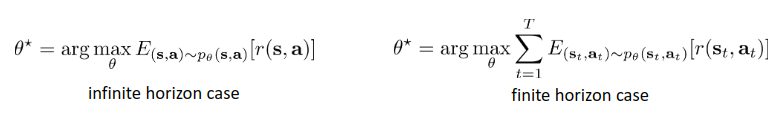
\includegraphics[scale=0.5]{cap3img/expectation2.png}
\end{center}
\caption{Finite Horizon}
\label{fig:horizon}
\end{figure}

\prettyref{fig:horizon} shows as we don't care about the reward of a particular trajectory, we care about the
expectation reward average over all the trajectories that could happen. Dealing with expectation is better because
expectation functions are smooth, and they are better to derivate. 


\subsection*{Slides 26-29}%
\label{sub:Slides 26-29}

\par Again, maximize the expectation of reward is what we want to. So, how do we deal with all this expectation?

Maximize: 
\begin{equation}
    \label{eq:expectation}
    \mathit{E}_{\tau \sim p_{\theta}(\tau)}\left [ \sum_{t=1}^{T}r(s_{t},a_{t}) \right] 
\end{equation}
\par We can express the equation \eqref{eq:expectation} as a recursive way:
\begin{equation}
        \begin{split}
        \mathit{E}_{\tau \sim p_{\theta}(\tau)}\left [ \sum_{t=1}^{T}r(s_{t},a_{t}) \right]  = 
        \mathit{E}_{s_{1} \sim p(s_{1})} \big[ \mathit{E}_{a_{1} \sim \pi(a_{1}|b_{1})} \\ \underbrace{\big[ r(s{1},a_{1}) +  
                \mathit{E}_{s_{2} \sim p(s_{2}|s_{1},a_{1})}\big[\mathit{E}_{a_{2} \sim \pi(a_{2}|s_{2})} \big[ 
    r(s_{2},a_{2}) + \cdots | s_{2}  \big]|s_{1},a_{1}\big]}_{Q(s_{1},a_{1})} |s_{1}\big]\big]
        \end{split}
\end{equation}

\par Simplified equation \eqref{eq:expectation} is:

\begin{equation}
    \mathit{E}_{\tau \sim p_{\theta}(\tau)}\left [ \sum_{t=1}^{T}r(s_{t},a_{t}) \right]  = \mathit{E}_{s_{1} \sim
    p(s_{1})} \big[ \mathit{E}_{a_{1} \sim \pi(a_{1}|s_{1})} \big[Q(s_{1},a_{1})|s_{1}\big]\big]
\end{equation}

If we know $Q(s_{1},a_{1})$, the policy can be modified to improve the reward expectation. For instance: Maximize the
likelihood of the action $a_{1}$ so that the probability of $\pi_{a_{x}|s_{1}} = 1$ if $a_{1} = argmax_{a_{1}} Q(s_{1},a_{1})$

\subsubsection*{Definition: Q-function}
\label{sub:Definition: Q-function}

$Q^{\pi}(s_{t},a_{t} = \sum_{t'=t}^{T} \mathit{E}_{\pi_{\theta}} \big[r(s_{t'},a_{t'})|s_{t},a_{t} \big]$: total reward
from taking $a_{t}$ in $s_{t}$ for the rest of the trajectory. Evaluate it  exactly is intractable, but it is possible to
use some algorithms to approximate Q-values. 

\subsubsection*{Definition: Value-Function}
\label{sub:Definition: Value-function}

It is similar to Q-Function, but not taking into account the action as input for calculations.

$V^{\pi}(s_{t}) = \sum_{t'=t}^{T} \mathit{E}_{\pi_{\theta}} \big[r(s_{t'},a_{t'})|s_{t} \big]$: total reward from
$s_{t}$. Using Q-function to express the Value-function: The sum of all actions  $Q(s_{t},a_{t})$(Expectation)
$V^{\pi}(s_{t}) = \mathit{E}_{a_{t} \sim \pi(a_{t}|s_{t})} \big[Q^{\pi}(s_{t},a_{t})\big]$. As a result, maximize the value in expectation of
at the first state, consequently maximizes the total expected reward of the entire policy. 
\begin{equation}
    \mathit{E}_{s_{1} \sim p(s_{1})}\big[V^{\pi}(s_{1})] \text{ is the RL objective!}
\end{equation}

\subsubsection*{How to use Q-Functions and Value-Functions to improve}
\label{sub:How to use Q-Functions and Value-Functions}

\begin{figure}
\begin{center}
    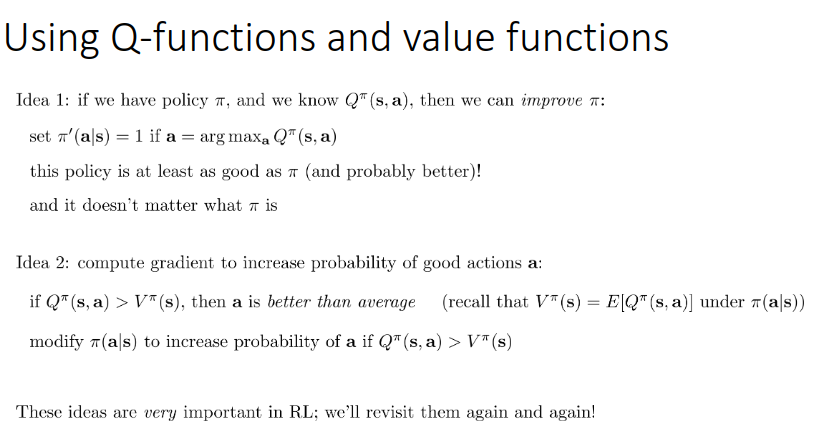
\includegraphics[scale=0.5]{cap3img/ideias.png}
\end{center}
\caption{Ideas to improve policy}
\label{fig:ideas}
\end{figure}

\par Idea 2 in \prettyref{fig:ideas} have been using in \textbf{actor-critic} models.


\section*{Slide 30-35}%
\label{sec:Slide 30-35}

\subsubsection*{Types of RL Algorithms}
\label{sub:Types of RL Algorithms}

\begin{equation}
        \label{eq:objective}
        \theta_{*} = \underset{\theta}{argmax}\mathit{E}_{\tau \sim p_{\theta}(\tau)} \Big[ \sum_{t}r_(s_{t},a_{t}) \Big] 
\end{equation}

\subsubsection*{Policy Gradients:}
\label{sub:Policy Gradients:}

\par Directly differentiate the equation \eqref{eq:objective}. Diagram in \prettyref{fig:Policy}

\begin{figure}
\begin{center}
    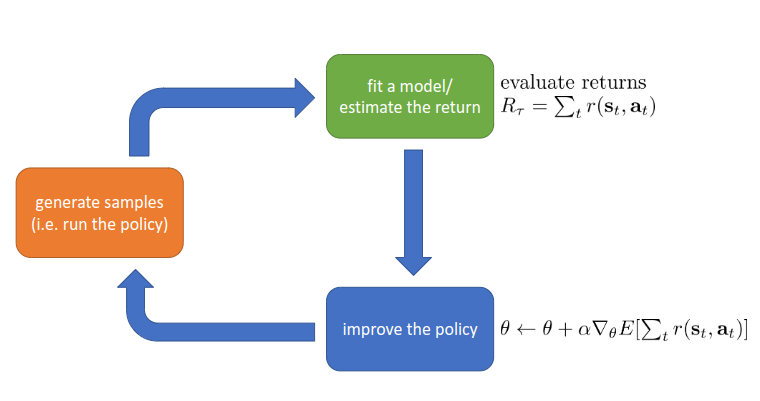
\includegraphics[scale=0.5]{cap3img/policy.png}
\end{center}
\caption{Policy-Gradients Diagram}
\label{fig:Policy}
\end{figure}



\subsubsection*{Value-Based}
\label{sub:Value-Based}

\par Estimate value function or Q-function of the optimal policy without representing the policy explicitly.  Only keep
tracking Q or V and improve these two functions through an iterative procedure. Diagram in \prettyref{fig:valuefunction}

\begin{figure}
\begin{center}
    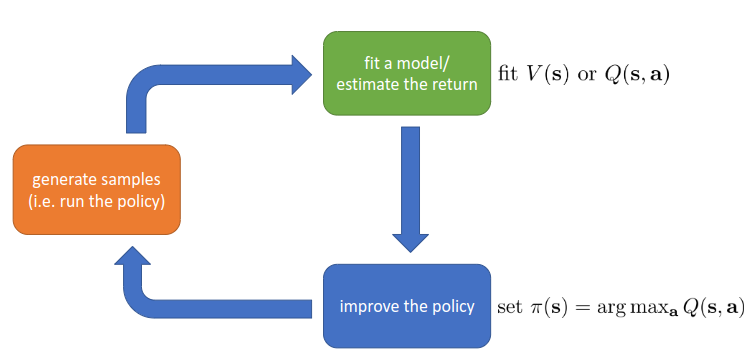
\includegraphics[scale=0.5]{cap3img/valurfunction.png}
\end{center}
\caption{Value-Function Diagram}
\label{fig:valuefunction}
\end{figure}


\subsubsection*{Actor-Critic}
\label{sub:Actor-Critic}

\par Combination of Policy Gradients and Value-Based. They estimate a value function or a Q-function and then 
improve it using something very similar to policy gradients. They calculate a gradient using value
functions and Q-functions. Diagram in \prettyref{fig:actor}

\begin{figure}
\begin{center}
    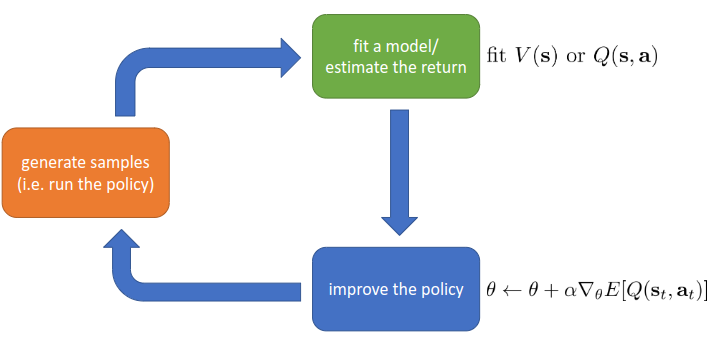
\includegraphics[scale=0.5]{cap3img/actor.png}
\end{center}
\caption{Actor-Critic Diagram}
\label{fig:actor}
\end{figure}

\subsubsection*{Model-Based RL}
\label{sub:Model-Based RL}

\par Estimate the transition model between states using $s_{t}$ and $a_{t}$. 
\begin{itemize}
    \item Use the model for planning(no explicit policy) - Optimal Control or Planning techniques
    \item Use the model to improve policy by pushing gradients or using the model to generate some synthetic
        experience and plugging it into more standard model-free RL algorithms, which maybe can be any of  this tree
        types of model above.
\end{itemize}

\par Diagram model-based RL in \prettyref{fig:modelbased}

\begin{figure}
\begin{center}
    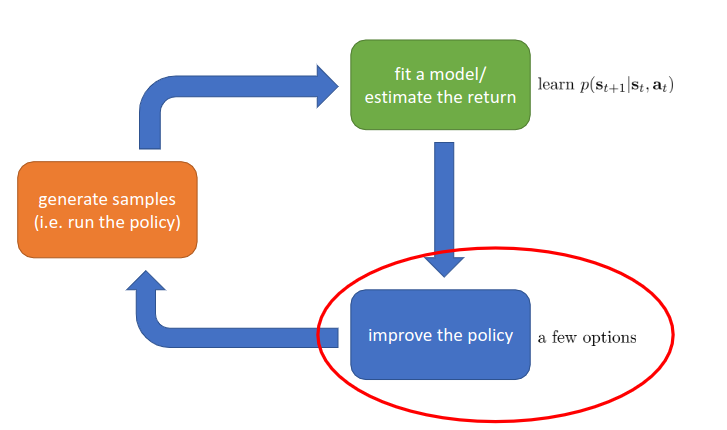
\includegraphics[scale=0.5]{cap3img/modelbasedrl.png}
\end{center}
\caption{Model-Based Diagram}
\label{fig:modelbased}
\end{figure}


\subsection*{Slide 36-43}%
\label{sub:Slide 36-43}

\subsubsection*{Tradeoffs}
\label{sub:Tradeoffs}

\begin{itemize}
    \item Different tradeoffs
        \begin{itemize}
            \item Sample Efficiency: How many times are necessary to run the policy to correct collect samples.
            \item Stability and ease of use.
        \end{itemize}
    \item Different assumptions
        \begin{itemize}
            \item Stochastic or deterministic?
            \item Continuous or discrete?
            \item Episodic or infinite horizon?
        \end{itemize}
    \item Different things are easy or had in different settings
        \begin{itemize}
            \item Easier to represent the policy?
            \item Easier to represent the model?
        \end{itemize}
\end{itemize}

\subsection*{Sample Efficiency}%
\label{sub:Sample Efficiency}

\begin{itemize}
    \item Sample efficiency: How many samples do we need to get a good policy? A sample means: Taking policy and run it
        and see what it does. 
    \item Is the algorithm \textit{off policy}?
        \begin{itemize}
            \item \textit{Off policy}: Able to improve the policy without generating new samples from that policy.
            \item \textit{On policy}: Each time the policy is changed, even a little bit, we need to generate new
                samples.
        \end{itemize}
\end{itemize}

\begin{figure}
\begin{center}
    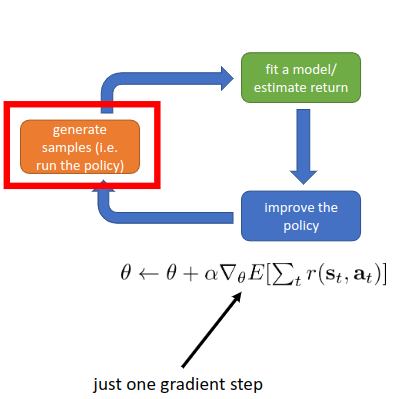
\includegraphics[scale=0.5]{cap3img/sample.png}
\end{center}
\caption{Sample Efficiency}
\label{fig:sample}
\end{figure}


\prettyref{fig:comparison} shows a comparison between different algorithms according to sample efficiency.

\begin{figure}
\begin{center}
    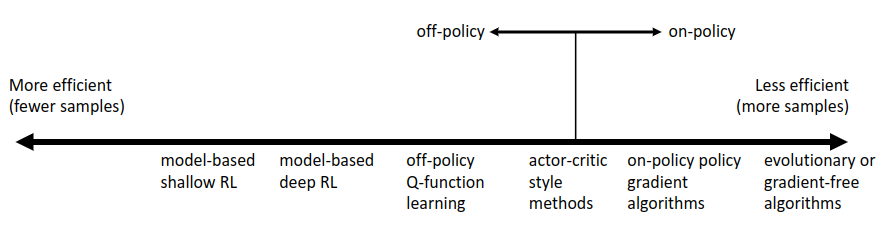
\includegraphics[scale=0.5]{cap3img/comparison.png}
\end{center}
\caption{Sample efficiency for different algorithms}
\label{fig:comparison}
\end{figure}

\subsubsection*{Stability and ease of use}
\label{sub:Stability and ease of use}

\begin{itemize}
    \item Does it converge? 
    \item And if it converges, to what?
    \item And does it converge every time?
    \item Supervised learning: Almost always gradient descent
    \item Reinforcement Learning: often not gradient descent
        \begin{itemize}
            \item Q-learning: Fixed Point Iteration
            \item Model-based RL: Model is not optimized for expected reward
            \item Policy Gradient: is gradient descent, but also often the least  efficient!
        \end{itemize}
\end{itemize}

\begin{itemize}
    \item Value function fitting
        \begin{itemize}
            \item At best, minimizes error of fit("Bellman error") 
                \begin{itemize}
                    \item Not the same as expected reward
                \end{itemize}
            \item At worst, doesn't optimize anything
                \begin{itemize}
                    \item Many popular deep RL value fitting algorithms are not guaranteed to converge to
                        anything in the nonlinear case.
                \end{itemize}
        \end{itemize}
    \item Model-based RL
        \begin{itemize}
            \item Model minimizes error fit
                \begin{itemize}
                    \item This will converge
                \end{itemize}
            \item Not guarantee that better model = better policy
        \end{itemize}
    \item Policy gradient
        \begin{itemize}
            \item The only one that actually performs gradient descent on the true objective.
        \end{itemize}
\end{itemize}

\subsubsection*{Assumptions}
\label{sub:Assumptions}

\begin{itemize}
    \item Common assumption \#1: Full Observability -  Seeing states and not observations
        \begin{itemize}
            \item Generally assumed by value function fitting methods
            \item Can be mitigate by adding recurrence
        \end{itemize}
    \item Common assumed \#2: Episodic Learning - Delimit of trials. 
        \begin{itemize}
            \item Often assumed by pure policy methods
            \item Assumed by some model-base RL methods
        \end{itemize}
    \item Common assumption \#3: Continuity or Smoothness
        \begin{itemize}
            \item Assumed by some continuous value function learning methods
            \item Often assumed by some model-based RL methods
        \end{itemize}
\end{itemize}

\subsubsection*{Examples of specific algorithms}
\label{sub:Examples of specific algorithms}

\begin{itemize}
    \item Value function fitting methods \begin{itemize}
        \item Q-learning, DQN
        \item Temporal difference learning
        \item Fitted value iteration
    \end{itemize}
    \item Policy gradient methods
        \begin{itemize}
            \item Reinforce
            \item Natural policy gradient
            \item Trust region policy optimization
        \end{itemize}
    \item Actor-critic algorithms
        \begin{itemize}
            \item Asynchronous advantage actor-critic (A3C)
            \item Soft actor-critic(SAC)
        \end{itemize}
    \item Model-based RL algorithms
        \begin{itemize}
            \item Dyna
            \item Guided policy search
        \end{itemize}
\end{itemize}


\end{document}
